\documentclass{article}
\usepackage[utf8]{inputenc}
\usepackage{amsmath}
\usepackage{amsthm}
\usepackage{amssymb}
\usepackage{amsfonts}
\usepackage{enumerate}
\usepackage{graphicx}
\usepackage{tikz}
\usetikzlibrary{matrix}
\usepackage[top=3cm,bottom=3cm,left=3.2cm,right=3.2cm,headsep=10pt,letterpaper]{geometry}

\newcommand{\R}{\mathbb{R}}
\newcommand{\C}{\mathbb{C}}
\newcommand{\N}{\mathbb{N}}
\newcommand{\Q}{\mathbb{Q}}
\newcommand{\I}{\mathbb{I}}


\newtheorem{theorem}{Teorema}
\newtheorem{definition}{Definição}


\title{Modelagem Matemática em Finanças I}
\author{Gil Sales Miranda Neto }
\date{2019}

\begin{document}
\begingroup
\thispagestyle{empty}
\tikz[remember picture,overlay] \node[inner sep=0pt] at (current page.center){
\includegraphics[width=\paperwidth,height=\paperheight]{background.jpg}};
\centering{
\textbf{\textcolor{black}{FODASE  }}}

\vspace*{1cm}
{\Huge \textcolor{black}{Curso ministrado por Prof. Marco Cabral - UFRJ 2019.1 \\ Gil Sales Miranda Neto}}\par % Author name
\endgroup
\newpage

\newpage
~\vfill
\thispagestyle{empty}
%\noindent Copyright \copyright\ 2014 Andrea Hidalgo\\ % Copyright notice

\noindent \textsc{Gil Sales Miranda Neto, Aluno de Graduação no Bacharelado em Matemática Aplicada - UFRJ}\\
Imagem da capa por Unsplash: https://unsplash.com/photos/R9OueKOtGGU\\
\noindent \textit{Última atualização \today} % Printing/edition date
\newpage
\section{Definindo termos}
\definition{\textbf{Não Arbitragem}}
Em um mercado que esteja tudo ocorrendo nos conforme, uma pessoa não encontrar uma oportunidade que seja sem risco e que pague mais do que a poupança. Esta é a teoria da não arbitragem. Arbitragem significa que você consegue encontrar uma oportunidade que é de baixissimo risco e altissima remuneração. Esse tipo de oportunidade não existe pois caso contrário, todo o mercado a usaria.
\\
Ou seja, é uma estratégia de investimento com zero probabilidade de perda e probabilidade positiva de lucro. Um modelo matemático que permite arbitragem não pode ser usado para análise.

\definition{\textbf{Preço de opções no modelo binomial}}
O inicio do periodo é chamado de \textit{tempo zero}. No tempo zero temos uma ação onde o preço por parte é dado por $S_0 > 0 \in \R$. Ao avançar o período para o tempo um, teremos um dos dois valores: $S_1(H)$ ou $S_1(T)$, onde H e T se referem a \textit{Head} e \textit{Tails}, do lançamento de moedas. Assumingo a probabilide de H: $p > 0$ e de T: $1 - p > 0$
$S_0 \to S_1(H) = uS_0$ ou $S_0 \to S_1(T) = dS_0$

\definition{\textbf{Up \& Down factors e Taxa de Juros}}\\
Definimos os números positivos
$$
u = \frac{S_1(H)}{S_0}
$$

$$
d = \frac{S_1(T)}{S_0}
$$

Como os fatores de subida e descida do valor da ação. Obviamente por definição temos $d < u$. Caso $d = u$, o valor da ação não é aleatório e o modelo não nos interessa.
\\
A taxa de juros $r$ significa que um dinheiro aplicado na poupança no tempo zero, irá render $1+r$ no tempo um. Obviamente definimos $r \geq 0$
\\
Para não haver arbitragem devemos assumir $0 < d < 1+r < u$

\theorem{Principio Fundamental da Contagem}

Considere dois experimentos $A_1$ e $A_2$, supondo que $A_1$ tenha $a_1$ possíveis resultados e $A_2$ tenha $a_2$
possíveis resultados, então o número de modos que os eventos $A_1$ e $A_2$ podemos ocorrem sucessivamente é $a_1\cdot a_2$

\\
inserir tree diagram e prova
\\

\theorem{Amostragem com reposição}
Considere n objetos e o evento de tomar k dentre estes n, onde se $n_i$ for tomado, pode ser tomado novamente num próximo experimento. Então há $n^k$ possíveis resultados.
\\
inserir prova
\\

\theorem{Amostragem sem repetição}
Considere n objetos e o experimento de tomar k dentre estes n objetos, onde se $n_i$ for resultado de um experimento, no próximo ele não pode ser tomado como resultado. Então há $n(n-1)\dots (n-k+1)$, com $n \geq k$

\subsection{O problema do aniversário}
Suponha que há k pessoas em uma sala. Assumindo que o aniversário de cada uma é equiprovavel para todos os 365 do ano. Qual a probabilidade de duas ou mais fazerem aniversário no mesmo dia?
\\
Pelo teorema 2, há $365^k$ combinações diferentes para distribuir os aniversários para k pessoas.\\
Como queremos que ao menos 2 pessoas compartilhem um dia de aniversário, vamos calcular o caso onde NINGUÉM compartilha nenhum aniversário, dai tomamos o complementar deste conjunto de eventos. Ou seja, se alguém faz aniversário em um dia, este dia não pode mais se repetir, aplicamos aqui o Teorema 2.
$365\cdot 364 \dots (365-k+1)$
\\
Tomando a probabilidade do evento A de ninguém compartilhar aniversário teremos
$$
P(A) = \frac{365\cdot 364 \dots (365-k+1)}{365^k}
$$
E a probabilidade do evento B, onde ao menos duas pessoas compartilham um aniversário
\begin{align*}
 P(B) = 1 - \frac{365\cdot 364 \dots (365-k+1)}{365^k}
\end{align*}
\\
\begin{figure}[h]
    \centering    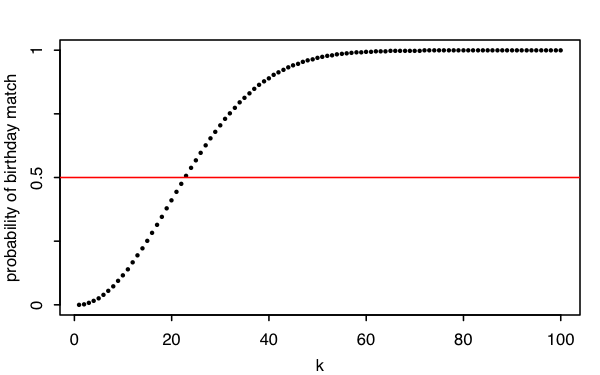
\includegraphics{fig1.png}
    \caption{Probabilidade de que em uma sala com $k$ pessoas, ao menos 2 tenham nascido no mesmo dia.}
    \label{fig:my_label}
\end{figure}
\end{document}
